%!TEX TS-program = xelatex
\documentclass{beamer}

\usepackage{HSE-theme/beamerthemeHSE} % Подгружаем тему

%%% Работа с русским языком и шрифтами
\usepackage[english,russian]{babel}   % загружает пакет многоязыковой вёрстки
\usepackage{fontspec}      % подготавливает загрузку шрифтов Open Type, True Type и др.
\defaultfontfeatures{Ligatures={TeX},Renderer=Basic}  % свойства шрифтов по умолчанию
\setmainfont[Ligatures={TeX,Historic}]{Myriad Pro} %  установите шрифты Myriad Pro или (при невозможности) замените здесь на другой шрифт, который есть в системе — например, Arial
\setsansfont{Myriad Pro}  %  установите шрифты Myriad Pro или (при невозможности) замените здесь на другой шрифт, который есть в системе — например, Arial
\setmonofont{Courier New}
\uselanguage{russian}
\languagepath{russian}
\deftranslation[to=russian]{Theorem}{Теорема}
\deftranslation[to=russian]{Definition}{Определение}
\deftranslation[to=russian]{Definitions}{Определения}
\deftranslation[to=russian]{Corollary}{Следствие}
\deftranslation[to=russian]{Fact}{Факт}
\deftranslation[to=russian]{Example}{Пример}
\deftranslation[to=russian]{Examples}{Примеры}

\usepackage{alltt}
\usepackage{multicol} 		% Несколько колонок
\graphicspath{{images/}}  	% Папка с картинками

\newfontfamily\dgmk[]{DejaVu Sans}
\newfontfamily\qgmk[Scale=MatchLowercase,Letters=SmallCaps]{Linux Libertine O}

%%% Информация об авторе и выступлении
\title[Disambiguation]{Morphological disambiguation} 
%\subtitle{Подзаголовок презентации / Название конференции}
\author[Francis M. Tyers]{Francis M. Tyers\\ \smallskip \scriptsize \url{ftyers@hse.ru}\\\url{https://www.hse.ru/org/persons/209454856}}
\institute[Высшая школа экономики]{Национальный исследовательский университет \\ «Высшая школа экономики» (Москва)}
\date{\today}

\begin{document}	% Начало презентации

\frame[plain]{\titlepage}	% Титульный слайд

\section{Просто слайд с текстом}
\subsection{Просто слайд с текстом}

\begin{frame}{Introduction}

% Orientation
% Tagsets 

\begin{itemize}
 \item Introduction, tagsets
 \item Approaches
 \begin{itemize}
    \item Rule-based
    \item HMM-based
    \item Averaged perceptron
 \end{itemize}
 \item Discussion
\end{itemize}

\end{frame}

\begin{frame}{Pipeline}

\begin{onlyenv}<1>
\includegraphics[width=\textwidth]{images/pipeline.eps}
\end{onlyenv}
\begin{onlyenv}<2>
\includegraphics[width=\textwidth]{images/pipeline-4.eps}
\end{onlyenv}

\end{frame}

\begin{frame}{Motivating example}

\begin{onlyenv}<1>
\begin{center}
{\LARGE {\bf при}}
\end{center}
\end{onlyenv}

% This I knew already from '46, when I started to write, and maybe even earlier -- and this
% fact more than once amazed me and left me in bewilderment about the usefulness of art
% inspite of the visibility of its impotence 
\begin{onlyenv}<3>
Это я знал еще с 46-го года, когда начал писать, а может быть и раньше,
-- и факт этот не раз поражал меня и ставил меня в  недоумение  о  полезности
искусства \textbf{при} таком видимом его бессилии.\\
~\\
\end{onlyenv}
\begin{onlyenv}<2->
\textbf{при:}  \\
\begin{itemize}
\item	\emph{при} ~ pr 
\item	\emph{пря} ~  n f nn sg gen 
\item	\emph{пря} ~  n f nn pl nom 
\item	\emph{пря} ~  n f nn pl acc 
\item	\emph{переть} ~  vblex impf tv imp p2 sg
\item	\emph{переть} ~  vblex impf iv imp p2 sg 
\end{itemize}
\end{onlyenv}
\end{frame}

\begin{frame}{Applications}

Aside from being a stage in the pipeline, what can use POS tagging directly ? 

\begin{itemize}
  \item \textbf{Speech synthesis}: How to pronounce a word in context, e.g. \emph{conduct}
  \begin{itemize}
     \item NOUN: /'kondukt/, VERB /kon'dukt/
  \end{itemize}
  \item \textbf{Disambiguation of meaning}:  
  \begin{itemize}
     \item lie NOUN vs. lie VERB
  \end{itemize}
  \item \textbf{Corpus linguistics}:
  \begin{itemize}
    \item Find sequences of lexical categories
    \item Limit searches for a wordform to a particular category
  \end{itemize}

\end{itemize}

% shallow syntactic representation

\end{frame}

\begin{frame}{Terminology}

% Part-of-speech tagging
% Morphological disambiguation
% Morphological analysis (~parsing)

\textbf{Part-of-speech tagging:}
   \begin{itemize}
     \item Traditional term, based on approach(es) for English, finite-set of 
       tags for all combinations of lexical category and morphology. \\ ~ \\
       \begin{tabular}{llllp{0.32\textwidth}}
         \hline
         \textbf{In:} & This & is & a & test \\
         ~ & This/PRON & is/VERB & a/DET & test/NOUN \\
         \hline
       \end{tabular}
   \end{itemize}
~\\
\textbf{Morphological disambiguation:}
   \begin{itemize}
      \item More cross-linguistically applicable, conception is of disambiguating
        after morphological analysis. \\  ~ \\
       \begin{tabular}{lllll}
         \hline
         \textbf{In:} & This/DET/PRON & is/VERB & a/DET & test/VERB/NOUN \\
         ~ & This/PRON & is/VERB & a/DET & test/NOUN \\
         \hline
       \end{tabular}
   \end{itemize}  

\end{frame}

\begin{frame}
\centering
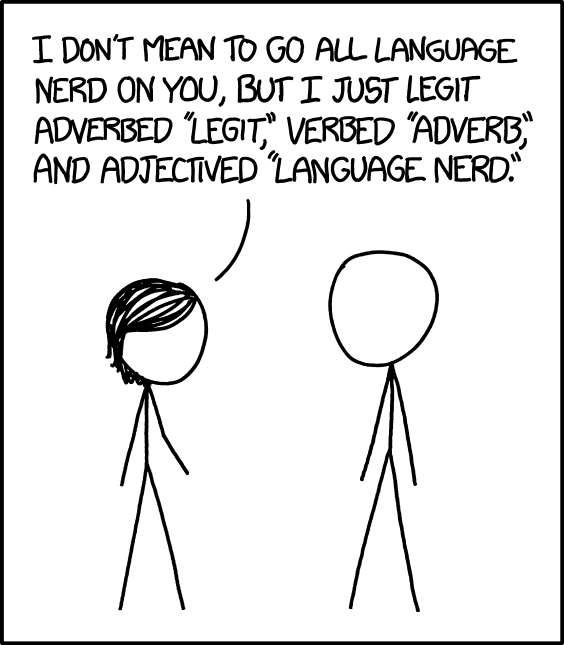
\includegraphics[width=0.7\textwidth]{images/language-nerd-2x.png}
\end{frame}

\begin{frame}{What is a tagset?}

\begin{itemize}
  \item Lemmas generalise over sets of inflectional forms
  \item Part-of-speech tags generalise over sets of lexemes/lemmas that have 
    similar syntactic distribution
\end{itemize}

\end{frame}

\begin{frame}{Tagset design}

\begin{columns}

\begin{column}{0.6\textwidth}

\textbf{Examples:}
\begin{itemize}
  \item Splitting: Participles from adjectives 
  \item Merging:  One class for all nominals
\end{itemize}
\textbf{Questions:}
\begin{itemize}
  \item Can the ambiguity be resolved? 
  \item Does the distinction help downstream applications?
\end{itemize}

\end{column}
\begin{column}{0.4\textwidth}
\begin{center}
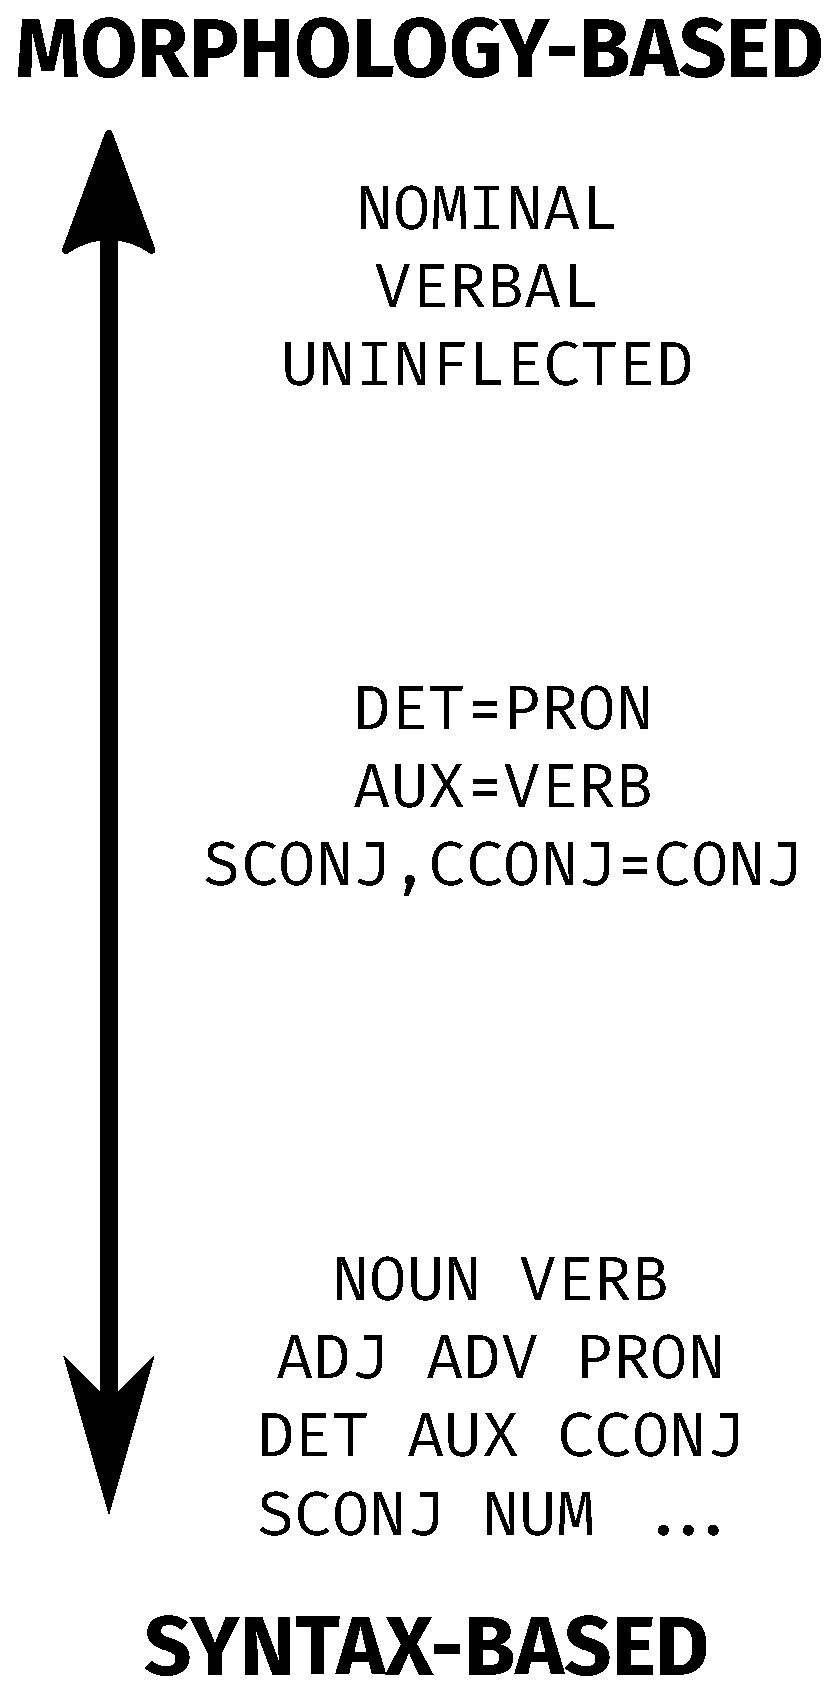
\includegraphics[width=0.7\textwidth]{images/tagset.eps}
\end{center}

\end{column}
\end{columns}

% Ambiguity
% 
% Morphological complexity % Language complexity tagging eng vs. chukchi

\end{frame}

\begin{frame}{Example tagsets}

%Penn Treebank style:
%Positional style:
%Universal Dependencies:
  
\begin{onlyenv}<1>
\begin{center}
\textbf{Penn Treebank} 
\end{center}
  \begin{columns}
  
    \begin{column}{0.4\textwidth}
    
    \begin{alltt}
       This/DT \\
       tagset/NNS  \\
       contains/VBZ \\
       48/CD \\
       unique/JJ \\
       tags/NNP  \\
       ./.  \\
    \end{alltt}
    
    \end{column}
    
    \begin{column}{0.6\textwidth}
    
    \begin{itemize}
       \item 48 tags 
       \item Tags are atomic
       \item Principles have been applied to other languages (Chinese, Bengali, \ldots)
       \item Extensible ? 
    \end{itemize}
    \end{column}

  \end{columns}
  
\end{onlyenv}

\begin{onlyenv}<2>
  \begin{center}
  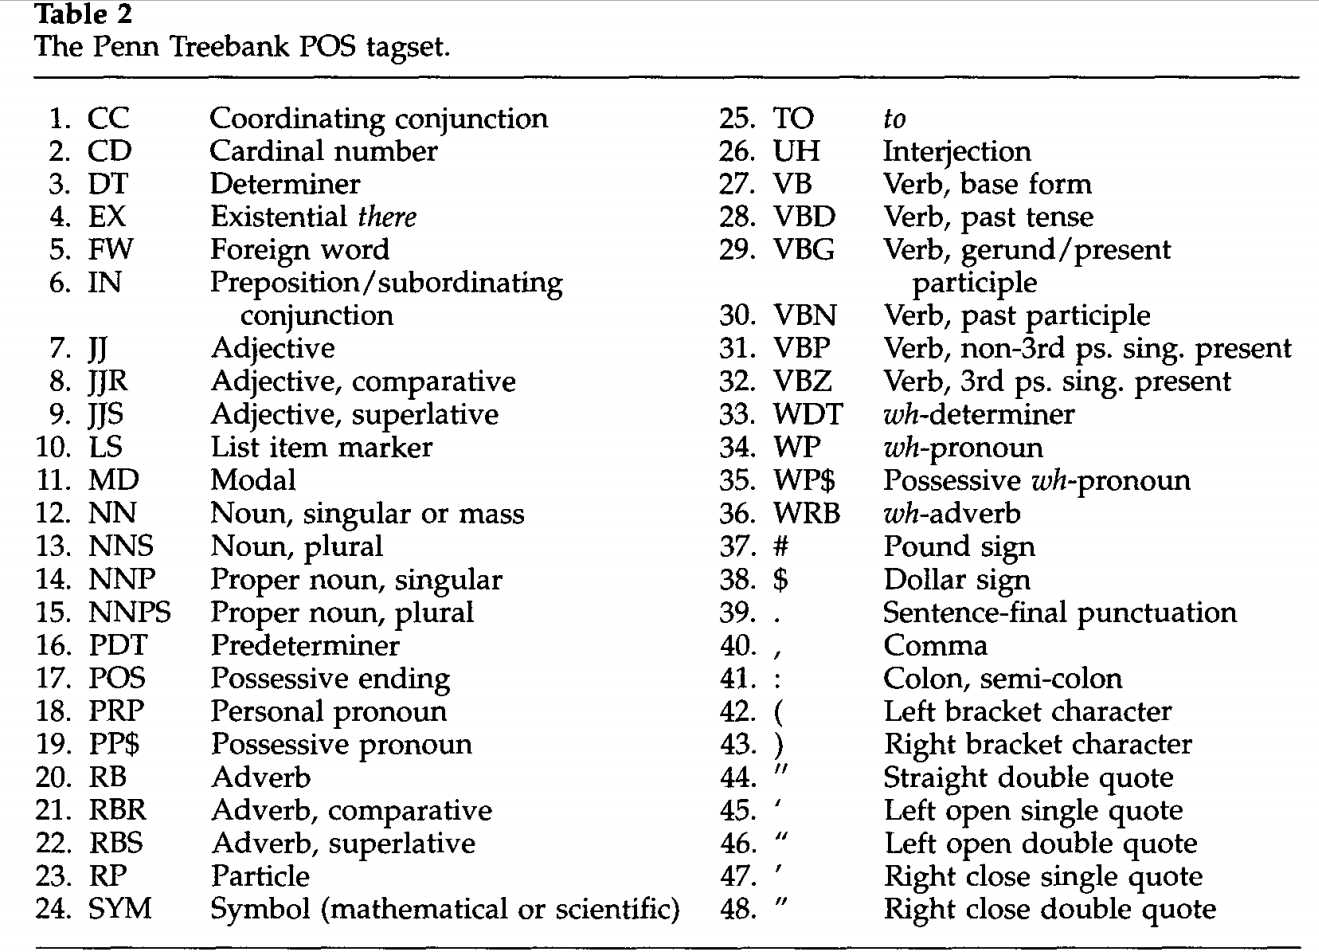
\includegraphics[width=0.9\textwidth]{images/penn-tagset.png}
  \end{center}
\end{onlyenv}

\begin{onlyenv}<3>
\begin{center}
\textbf{Positional tags} 
~\\
~\\

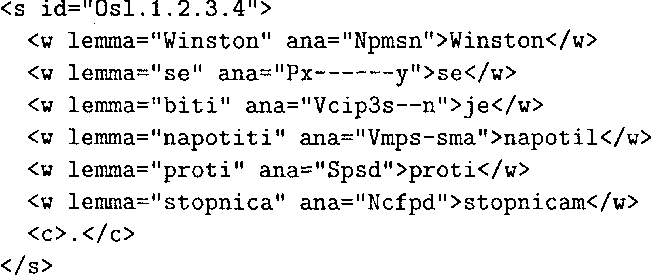
\includegraphics[width=0.7\textwidth]{images/12-Figure5-1.png}
\end{center}

\begin{itemize}
 \item[+] Compact
 \item[-] Hard to read 
 \item[-] No support for derivational morphology
\end{itemize}

\end{onlyenv}

\begin{onlyenv}<4>
\begin{center}
\textbf{Mnemonic tags} 

\end{center}
{\tiny
\begin{alltt}
Sápmelaččas	[sápmelaš] N Sg Loc \\
leai	[leat] V IV Ind Prt Sg3 \\
dakkár	[dakkár] Pron Dem Attr \\
luondu	[luondu] N Sg Nom \\
,	[,] CLB \\
ahte	[ahte] CS \\
son	[son] Pron Pers Sg3 Nom \\
háliidišgođii	[háliidit] V TV Der/goahti Ind Prt Sg3 \\
gottiid	[goddi] N Pl Acc \\
.	[.] CLB \\
\end{alltt}
}
\begin{itemize}
  \item[+] Easily handle derivations
  \item[+] Implicit morphological structure
  \item[-] Number of tags can explode
  \item[-] Modelling derivation is less language-independent
\end{itemize}

\end{onlyenv}

\begin{onlyenv}<5>
\begin{center}
\textbf{Feature/value pairs} 
\end{center}
\begin{center}
\scalebox{0.7}{
\begin{tabular}{lllllll}
1  & Польша & \_& PROPN & \_& Animacy=Inan|Case=Nom|Gender=Fem|Number=Sing & \_   \\
2  & является & \_& VERB & \_& Aspect=Imp|Number=Sing|Person=3|Tense=Pres & \_   \\
3  & безъядерной & \_& ADJ & \_& Animacy=Inan|Case=Ins|Gender=Fem|Number=Sing & \_ \\
4  & страной & \_& NOUN & \_& Animacy=Inan|Case=Ins|Gender=Fem|Number=Sing & \_ \\
5  & . & \_& PUNCT & \_& \_ & \_ \\
\end{tabular}
}
\end{center}

\begin{itemize}
 \item[+] Easy to read
 \item[-] No support for derivational morphology
 \item[-] No implicit morphological structure
 \item[-] Takes up a lot of space 
\end{itemize}

\end{onlyenv}

\end{frame}

% Tagset considerations morph<-->syntax

\begin{frame}{Limitations}

\begin{center}
\fbox{
  \begin{minipage}[t]{0.7\textwidth}
\dgmk{ӄорагыркиплыткогъат} 
\begin{itemize}
  \item \dgmk{ӄора-гырки-плыткогъат} \\
  \item reindeer-catch-finish-{\sc 3PL} \\
  \item \emph{They finished catching reindeer.}
\end{itemize}
\end{minipage}
}
\end{center}

\begin{itemize}
  \item Does \texttt{VERB} really capture what this is ?
  \item We can represent morphology easily, maybe even derivation
  \item But what about the incorporation ?
\end{itemize}



\end{frame}

\begin{frame}{Scale of the problem}
% scale of the problem (how many words are ambiguous?) types/tokens

\begin{columns}
\begin{column}{0.4\textwidth}

\begin{itemize}
  \item UD corpora
  \item Percentage of tokens and types that receive more than
    one analysis 
  \item Underestimation, e.g. Turkish \emph{için}:
  \begin{itemize}
    \item[+] for.{\sc POST} 
    \item[+] inside.{\sc GEN}
    \item[-] inside.{\sc 2SG.NOM}
    \item[-] drink.{\sc IMP.2PL}
  \end{itemize}
\end{itemize}

\end{column}
\begin{column}{0.6\textwidth}
    \begin{tabular}{lrrr}
    \textbf{Language} & \textbf{Tokens} & \textbf{/type} & \textbf{/token} \\
    \hline
    Turkish   & 58k &  4.29    &  17.44 \\
    Finnish   & 201k &  3.46   &  18.09 \\
    Kurmanji   & 10k&  9.35    &  36.72 \\
    Basque   & 121k&  11.47    &  38.47 \\
    Russian  & 1.1M &  13.50    &  40.94 \\
    Erzya   & 2k &  9.73   &   41.37 \\
    Norwegian  & 301k &  8.28    &  43.78 \\
    Czech   & 1.5M &  18.09   &   47.17 \\
    English   & 254k &  14.20    &  52.34 \\
    German   & 292k &  20.17    &  56.52 \\
    Portuguese  & 227k&  13.19    &  64.51 \\
    Catalan   & 531k &  8.31   &  66.49 \\
    Hebrew   & 161k &  15.56   &  71.62 \\
    Hindi   & 351k &  36.28   &  86.84 \\
    \hline
    \end{tabular}
    
\end{column}

\end{columns}

\end{frame}

\begin{frame}{Types of ambiguity}
% Morphological ambiguity ... types

\begin{center}
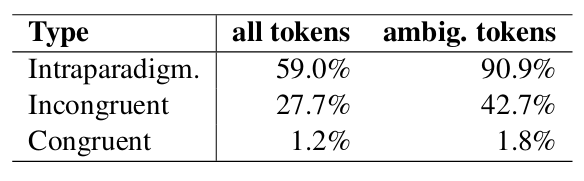
\includegraphics[width=0.7\textwidth]{images/ambig-types.png}
\end{center}

\begin{itemize}
  \item Intraparadigmatic:
  \begin{itemize}
    \item 'тела (SG.GEN) vs. тел'а (PL.NOM)
  \end{itemize}
  \item Morphosyntactically incongruent:
  \begin{itemize}
    \item до'рога (NOUN) vs. дорог'а (ADJ)
  \end{itemize}
  \item Morphosyntactically congruent:
  \begin{itemize}
    \item 'замок (SG.NOM) vs. зам'ок (SG.NOM)
  \end{itemize}
\end{itemize}

\end{frame}

%\begin{frame}{A baseline}
% most freq. class baseline

%\end{frame}

% what POS tagging is not... tokenisation/multiwords

% Applications


\begin{frame}{Approaches}
% Approaches

\begin{itemize}
   \item \textbf{Rule-based} 
   \item \textbf{HMM-based} 
   \item \textbf{Averaged perceptron}
\end{itemize}

\end{frame}

%%%%%%%%%%%%%%%%%%%%%%%%%%%%%%%%%%%%%%%%%%%%%%%%%%%%%%%%%%%%%%%%%%%%%%%%%%%%%%%
%% Rule-based ... CG, ...
\begin{frame}
\centering
{\LARGE {\bf Rule-based } }
\end{frame}

\begin{frame}{Constraint Grammar}

    \begin{itemize}
      \item Developed by Fred Karlsson\footnote{The same Fred Karlsson that wrote ``Finsk grammatik''.} in the late 1980s
      \item Does not aim at producing a full ``parse tree''
      \item Describes what is \emph{ungrammatical}, not what is grammatical
      \item Linguists formalise ``constraints'' which describe language impossibilities
      \begin{itemize}
        \item e.g. ``No noun can be in prepositional case without a preposition which 
          governs the prepositional case.''
      \end{itemize}
      \item No ``encapsulation'', all parts of the analysis (surface form $\rightarrow$ semantics) are always available
      \item Input is all possible analyses, output is only possible analyses
    \end{itemize}

\end{frame}

\begin{frame}{Formalism}

\begin{columns}
\column{.45\textwidth}
   \textbf{Input:}
\begin{tiny}
\begin{alltt}
"<Польша>"\\
~~~~"Польша" np top f sg nom\\
"<является>"\\
~~~~"являться" v impf iv pres p3 sg\\
"<безъядерной>"\\
~~~~"безъядерный" adj f an sg gen\\
~~~~"безъядерный" adj f an sg dat\\
~~~~"безъядерный" adj f an sg prp\\
~~~~"безъядерный" adj f an sg ins\\
"<страной>"\\
~~~~"страна" n f nn sg ins\\
"<.>"\\
~~~~"." sent\\
\end{alltt}
\end{tiny}

\column{.55\textwidth}
   \textbf{Operators:}
     \begin{itemize}
       \item {\sc select}: \dgmk{Discard all readings except the reading matching a condition}
       \item {\sc remove}: \dgmk{Discard a single reading matching a condition}
     \end{itemize}
\end{columns}

~\\
~\\
\noindent
   \textbf{Context conditions:}
     \begin{itemize}
       \item \dgmk{(-1 pres)} $\rightarrow$ previous token has the tag \qgmk{pres} 
       \item \dgmk{(1C ins)} $\rightarrow$ following token \emph{only} has the tag \qgmk{ins}
       \item \dgmk{(NOT -1* pr)} $\rightarrow$ no token to the left has the tag \qgmk{pr}
     \end{itemize}


\end{frame}

\begin{frame}{Basic example}

\begin{columns}
\column{.45\textwidth}
   \textbf{Input:}
\begin{tiny}
\begin{alltt}
"<Польша>"\\
~~~~"Польша" np top f sg nom\\
"<является>"\\
~~~~"являться" v impf iv pres p3 sg\\
"<безъядерной>"\\
\alert<3-4>{~~~~"безъядерный" adj f an sg gen}\\
\alert<4>{~~~~"безъядерный" adj f an sg dat}\\
\alert<2-4>{~~~~"безъядерный" adj f an sg prp}\\
~~~~"безъядерный" adj f an sg ins\\
"<страной>"\\
~~~~"страна" n f nn sg ins\\
"<.>"\\
~~~~"." sent\\
\end{alltt}
\end{tiny}

\column{.55\textwidth}
\begin{onlyenv}<2>
\begin{itemize}
  \item[1] \qgmk{remove} \dgmk{prp} \qgmk{if} \dgmk{(not -1* pr)}
\end{itemize}
\end{onlyenv}
\begin{onlyenv}<3->
\begin{itemize}
  \item[1] \qgmk{remove} \dgmk{prp} \qgmk{if} \dgmk{(not -1* pr)}
  \item[2] \qgmk{remove} \dgmk{gen} \qgmk{if} \dgmk{(-1 pres) (0C adj) (not 1 gen)}
\end{itemize}
\end{onlyenv}

\end{columns}

\begin{onlyenv}<4>
~\\
~\\
Exercise: Can we safely remove the dative reading?
\end{onlyenv}

\end{frame}

\begin{frame}{Less basic example}

 \begin{large}
 « Для соседних с Руандой государств руандийские события апреля – июля 1994 года вылились в огромное число прибывших беженцев . »
 \end{large}
 % russian example

\end{frame}

\begin{frame}
  \frametitle{Standard trigram taggers}

    \begin{tiny}
        \begin{tabular}{ll}
        Для & PR  \\
        соседних & A=pl,gen,plen  \\
        с & PR  \\
        Руандой & S,f,inan=sg,ins  \\
        государств & S,n,inan=pl,gen  \\
        руандийские & \alert<2>{A=pl,acc,inan,plen}  \\
        события & \alert<2>{S,n,inan=pl,acc}  \\
        апреля & S,m,inan=sg,gen  \\
        – & –  \\
        июля & S,m,inan=sg,gen  \\
        1994 & NUM=ciph  \\
        года & S,m,inan=sg,gen  \\
        вылились & V,pf,intr,med=pl,praet,indic  \\
        в & PR  \\
        огромное & A=n,sg,acc,inan,plen  \\
        число & S,n,inan=sg,acc  \\
        прибывших & V,pf,intr,act=partcp,pl,gen,praet,plen  \\
        беженцев & S,m,anim=pl,gen  \\
        . & .  \\
        \end{tabular}
    \end{tiny}

    \begin{onlyenv}<1>
    ~\\
    ~\\
    \end{onlyenv}
    \begin{onlyenv}<2>
    ~\\
    \begin{flushright}
    2 / 19 = 89.5\% accuracy
    \end{flushright}
    \end{onlyenv}
    
\end{frame}

\begin{frame}{Input: Morphological analysis}

  \begin{flushright}
    \begin{tiny}
      \begin{onlyenv}<1>
        rule: --
      \end{onlyenv}
      \begin{onlyenv}<2>
        rule: 1
      \end{onlyenv}
      \begin{onlyenv}<3>
        rule: 2
      \end{onlyenv}
      \begin{onlyenv}<4>
        rule: 3
      \end{onlyenv}
      \begin{onlyenv}<5>
        rule: 4
      \end{onlyenv}
      \begin{onlyenv}<6-7>
        rule: 5
      \end{onlyenv}
    \end{tiny}
  \end{flushright}
\vspace{-40.0pt}
\begin{columns}
\column{.45\textwidth}
  \begin{tiny}
     \begin{alltt}
"<Для>"\\
\alert<2>{~~~"для" pr}
~\\
"<соседних>"\\
\alert<2>{~~~"соседний" adj mfn an pl gen} \\
\begin{onlyenv}<1>
~~~"соседний" adj mfn an pl prp\\
~~~"соседний" adj mfn aa pl acc
\end{onlyenv}
\begin{onlyenv}<2->
\textcolor{lightgray}{
~~~"соседний" adj mfn an pl prp\\
~~~"соседний" adj mfn aa pl acc
}
\end{onlyenv}
~\\
"<с>"\\
~~~"с" pr
~\\
"<Руандой>"\\
~~~"Руанда" np top f sg ins
~\\
"<государств>"\\
~~~"государство" n nt nn pl gen
~\\
"<руандийские>"\\
\alert<5>{~~~"руандийский" adj mfn an pl nom}\\
\begin{onlyenv}<1-4>
~~~"руандийский" adj mfn nn pl acc
\end{onlyenv}
\begin{onlyenv}<5->
\textcolor{lightgray}{
~~~"руандийский" adj mfn nn pl acc
}
\end{onlyenv}
~\\
"<события>"\\
\begin{onlyenv}<1-4>
~~~"событие" n nt nn sg gen\\
\end{onlyenv}
\begin{onlyenv}<5->
\textcolor{lightgray}{
~~~"событие" n nt nn sg gen\\
}
\end{onlyenv}
\alert<5>{~~~"событие" n nt nn pl nom}\\
\begin{onlyenv}<1-3>
~~~"событие" n nt nn pl acc
\end{onlyenv}
\begin{onlyenv}<4->
\textcolor{lightgray}{
~~~"событие" n nt nn pl acc
}
\end{onlyenv}
~\\
"<апреля>"\\
~~~"апрель" n m nn sg gen
~\\
"<–>"\\
~~~"–" guio
~\\
"<июля>"\\
~~~"июль" n m nn sg gen
~\\
    \end{alltt}
  \end{tiny}
  \column{.55\textwidth}
    \begin{tiny}
      \begin{alltt}
    "<1994>"\\
    ~~~"1994" num
    ~\\
    "<года>"\\
    ~~~"год" n m nn sg gen\\
    "<вылились>"\\
    \alert<4,5>{~~~"вылиться" v perf iv past mfn pl}
    ~\\
    "<в>"\\
    \alert<3>{~~~"в" pr}
    ~\\
    "<огромное>"\\
    \begin{onlyenv}<1-2>
    ~~~"огромный" adj nt an sg nom\\
    \end{onlyenv}
    \begin{onlyenv}<3->
    \textcolor{lightgray}{
    ~~~"огромный" adj nt an sg nom\\
    }
    \end{onlyenv}
    \alert<3>{~~~"огромный" adj nt an sg acc}
    ~\\
    "<число>"\\
    \alert<3,6>{~~~"число" n nt nn sg acc}\\
    \begin{onlyenv}<1-2>
    ~~~"число" n nt nn sg nom
    \end{onlyenv}
    \begin{onlyenv}<3->
    \textcolor{lightgray}{
    ~~~"число" n nt nn sg nom
    }
    \end{onlyenv}
    ~\\
    "<прибывших>"\\
    \begin{onlyenv}<1-3>
    ~~~"прибыть" v perf iv pp actv mfn an pl acc  \\
    \end{onlyenv}
    \begin{onlyenv}<4->
    \textcolor{lightgray}{
    ~~~"прибыть" v perf iv pp actv mfn an pl acc  \\
    }
    \end{onlyenv}
    \begin{onlyenv}<1-6>
    \alert<6>{~~~"прибыть" v perf iv pp actv mfn an pl prp} \\
    \end{onlyenv}
    \begin{onlyenv}<7->
    \textcolor{lightgray}{
    ~~~"прибыть" v perf iv pp actv mfn an pl prp \\
    }
    \end{onlyenv}
    \begin{onlyenv}<1-7>
    ~~~"прибыть" v perf iv pp actv mfn aa pl gen
    \end{onlyenv}
    ~\\
    "<беженцев>"\\
    \alert<4>{~~~"беженец" n m aa pl gen}\\
    \begin{onlyenv}<1-3>
    ~~~"беженец" n m aa pl acc
    \end{onlyenv}
    \begin{onlyenv}<4->
    \textcolor{lightgray}{
    ~~~"беженец" n m aa pl acc
    }
    \end{onlyenv}
    ~\\
    "<.>"\\
    ~~~"." sent
    \end{alltt}
    \end{tiny}

    \end{columns}
%!%
\end{frame}

\begin{frame}
  \frametitle{Proposed rule (I)}

  \begin{itemize}
    \item[1] Immediately after ``для'' remove any reading which is in a case other 
       than genitive.
  \end{itemize}
~\\
\textbf{Exceptions:}
  \begin{itemize}
    \item None ? 
  \end{itemize}
~\\
\textbf{Formalised:}

{\small
\begin{alltt}
  LIST Gen = gen ; \\
  SET NGDAIP = nom OR gen OR dat OR acc OR ins OR prp ;  \\
  REMOVE NGDAIP - Gen IF (-1C ("для")) ; \\
\end{alltt}
}
\end{frame}

\begin{frame}
  \frametitle{Proposed rule (II)}
 
  \begin{itemize}
    \item[2] After ``в'' remove any reading which is in nominative % certain constructions allow this ?

  \end{itemize}

~\\
\textbf{Exceptions:}
  \begin{itemize}
    \item Joining an organisation ?
  \end{itemize}

~\\
\textbf{Formalised:}
{\small
\begin{alltt}
  LIST Nom = nom ; \\
  REMOVE Nom IF (-1C ("в")) ;
\end{alltt}
}
\end{frame}

\begin{frame}
  \frametitle{Proposed rule (III)}

  \begin{itemize}
    \item[3] In a sentence with a single intransitive finite verb, remove any reading in accusative which is not
       immediately governed by a preposition % or transitive participle form or some adverbial forms ?
  \end{itemize}

~\\
\textbf{Exceptions:}
  \begin{itemize}
    \item There is a trans. part. form having an acc. arg.
    \item Some adverbial forms... \emph{Мы проехали километр.}
  \end{itemize}

~\\
\textbf{Formalised:}
{\small
  \begin{alltt}
  LIST IV = iv ; \\
  LIST TV = tv ; \\
  LIST Acc = acc ; \\
  LIST Pr = pr ; \\
  REMOVE Acc IF (0 Acc LINK NOT -1* Pr) ((-1* IV) OR (1* IV)) (0 Acc LINK NOT 1* TV) (0 Acc LINK NOT -1* TV) ; 
  \end{alltt}
}
\end{frame}
  
\begin{frame}
  \frametitle{Proposed rule (IV)}

  \begin{itemize}
    \item[4] Select nominative if there is an intransitive verb which agrees with a nominative noun in the sentence 
       for number (and/or gender)
     \begin{itemize}
        \item and is preceeded by an adj. that can only be nom.
        \item and there is no other nom. head in the sentence.
     \end{itemize}
  \end{itemize}
~\\
\textbf{Exceptions:}
  \begin{itemize}
    \item Appositions, titles, parentheticals ? Non-canonical agreement ?
  \end{itemize}
~\\
\textbf{Formalised:}
{\small
  \begin{alltt}
    LIST Head = np n prn ;\\
    SET NUM = (sg) OR (pl) ; \\
    SELECT Nom + \$\$NUM IF (-1C A + Nom) (NOT -1* Head + Nom) (NOT 1* Head + Nom) ((-1* V + \$\$NUM) OR (1* V + \$\$NUM));
  \end{alltt}
}
\end{frame}

\begin{frame}
  \frametitle{Proposed rule (V)}

  \begin{itemize}
    \item[5] If there is a prepositional case reading, remove it if you see a
       noun which is only in a case other than prepositional without any preceeding transitive participle form
  \end{itemize}
~\\
\textbf{Exceptions:}
  \begin{itemize}
    \item ...
  \end{itemize}

~\\
\textbf{Formalised:}
{\small
  \begin{alltt}
    LIST Prp = prp ; \\
    LIST N = n ;\\
    REMOVE Prp IF (-1* N + NGDAIP - Prp) ;\\
  \end{alltt}
}

\end{frame}

\begin{frame}
    \frametitle{Output: Morphologically-disambiguated text}

\begin{columns}
\column{.45\textwidth}
\begin{tiny}
\begin{alltt}
"<Для>"\\
~~~"для" pr
~\\
"<соседних>"\\
~~~"соседний" adj mfn an pl gen\\
\textcolor{lightgray}{
~~~"соседний" adj mfn an pl prp\\
~~~"соседний" adj mfn aa pl acc
}
~\\
"<с>"\\
~~~"с" pr
~\\
"<Руандой>"\\
~~~"Руанда" np top f sg ins
~\\
"<государств>"\\
~~~"государство" n nt nn pl gen
~\\
"<руандийские>"\\
~~~"руандийский" adj mfn an pl nom\\
\textcolor{lightgray}{
~~~"руандийский" adj mfn nn pl acc
}

~\\
"<события>"\\
\textcolor{lightgray}{
~~~"событие" n nt nn sg gen\\
}
~~~"событие" n nt nn pl nom\\
\textcolor{lightgray}{
~~~"событие" n nt nn pl acc
}

~\\
"<апреля>"\\
~~~"апрель" n m nn sg gen
~\\
"<–>"\\
~~~"–" guio
~\\
"<июля>"\\
~~~"июль" n m nn sg gen
~\\
\end{alltt}
\end{tiny}
\column{.55\textwidth}
\begin{tiny}
\begin{alltt}
"<1994>"\\
~~~"1994" num
~\\
"<года>"\\
~~~"год" n m nn sg gen\\
"<вылились>"\\
~~~"вылиться" v perf iv past mfn pl
~\\
"<в>"\\
~~~"в" pr
~\\
"<огромное>"\\
\textcolor{lightgray}{
~~~"огромный" adj nt an sg nom\\
}
~~~"огромный" adj nt an sg acc
~\\
"<число>"\\
~~~"число" n nt nn sg acc\\
\textcolor{lightgray}{
~~~"число" n nt nn sg nom
}

~\\
"<прибывших>"\\
\textcolor{lightgray}{
~~~"прибыть" v perf iv pp actv mfn an pl acc  \\
~~~"прибыть" v perf iv pp actv mfn an pl prp \\
}
~~~"прибыть" v perf iv pp actv mfn aa pl gen
~\\
"<беженцев>"\\
~~~"беженец" n m aa pl gen\\
\textcolor{lightgray}{
~~~"беженец" n m aa pl acc
}

~\\
"<.>"\\
~~~"." sent
\end{alltt}
\end{tiny}
\end{columns}

\end{frame}
%
%\begin{frame}{Rule application}
%
%
%\end{frame}
%
%\begin{frame}{Effort}
%
%% Trosterud: 
%% Huldén:
%% Tyers (Breton)
%% Tyers (Russian)
%% Voutilainen:
%
%\end{frame}
%
%\begin{frame}{Cost / benefit}
%
%%
%%% no need for annotated corpus
%%% more interesting than manually annotating a tonne of text
%
%% 
%%% problems with tagset changes
%
%
%\end{frame}

\begin{frame}{Examples}

Languages with constraint grammars:
\begin{itemize}
  \item Finnish
  \item North Sámi, Lule Sámi, South Sámi
  \item Norwegian (Nynorsk, Bokmål)
  \item Faroese
  \item Udmurt
  \item Breton
\end{itemize}

\end{frame}

%% Rule-application

%%%%%%%%%%%%%%%%%%%%%%%%%%%%%%%%%%%%%%%%%%%%%%%%%%%%%%%%%%%%%%%%%%%%%%%%%%%%%%%
% HMM
\begin{frame}
\centering
{\LARGE {\bf HMM-based } }
\end{frame}

% generative model
\begin{frame}


Predict hidden states from observed events
\begin{itemize}
\item hidden states = sequence of part of speech tags
\item observed events = ambiguity classes or surface forms
\end{itemize}
~\\
\begin{center}
{\Large $M = (A, B, \pi)$}
\end{center}
~\\
\begin{itemize}
  \item $A$ = transition probabilities
  \item $B$ = emission probabilities
  \item $\pi$ = initial probabilities
\end{itemize}

\end{frame}

% assumptions

% bigrams

\begin{frame}{Visible events}

The visible events can be either:

\begin{itemize}
  \item \textbf{Surface forms:} In many traditional HMM-based taggers, the visible events are 
    surface forms
  \item \textbf{Ambiguity classes:} Generalisation over types of ambiguity e.g. NOUN/VERB, DET/PRON
\end{itemize}

Example:
\begin{center}
\scalebox{0.9}{
\begin{tabular}{llllll}
Surface forms: &   This &  is &  a &  test & .  \\
Ambig. classes: & PRON/DET & VERB/AUX & DET & VERB/NOUN & PUNCT \\
\end{tabular}
}
\end{center}

\end{frame}

% worked example

\begin{frame}{A tagged corpus}

\textbf{Analysed:} \\
\begin{tabular}{ll}
& Vino/\textcolor{gray}{NOUN}/\textcolor{gray}{VERB} a/\textcolor{gray}{ADP} la/\textcolor{gray}{DET}/\textcolor{gray}{PRON} playa/\textcolor{gray}{NOUN} ./\textcolor{gray}{PUNCT} \\
& Voy/\textcolor{gray}{VERB} a/\textcolor{gray}{ADP} la/\textcolor{gray}{DET}/\textcolor{gray}{PRON} casa/\textcolor{gray}{NOUN}/\textcolor{gray}{VERB} ./\textcolor{gray}{PUNCT} \\
& Bebe/\textcolor{gray}{VERB} vino/\textcolor{gray}{NOUN}/\textcolor{gray}{VERB} en/\textcolor{gray}{ADP} casa/\textcolor{gray}{NOUN}/\textcolor{gray}{VERB} ./\textcolor{gray}{PUNCT} \\
& La/\textcolor{gray}{DET}/\textcolor{gray}{PRON} casa/\textcolor{gray}{NOUN}/\textcolor{gray}{VERB} es/\textcolor{gray}{VERB} grande/\textcolor{gray}{ADJ} ./\textcolor{gray}{PUNCT} \\
& Es/\textcolor{gray}{VERB} una/\textcolor{gray}{DET}/\textcolor{gray}{PRON}/\textcolor{gray}{VERB} ciudad/\textcolor{gray}{NOUN} grande/\textcolor{gray}{ADJ} ./\textcolor{gray}{PUNCT} \\
\end{tabular} 

\textbf{Tagged:} \\
\begin{tabular}{ll}
& Vino/\textcolor{gray}{VERB} a/\textcolor{gray}{ADP} la/\textcolor{gray}{DET} playa/\textcolor{gray}{NOUN} ./\textcolor{gray}{PUNCT} \\
& Voy/\textcolor{gray}{VERB} a/\textcolor{gray}{ADP} la/\textcolor{gray}{DET} casa/\textcolor{gray}{NOUN} ./\textcolor{gray}{PUNCT} \\
& Bebe/\textcolor{gray}{VERB} vino/\textcolor{gray}{NOUN} en/\textcolor{gray}{ADP} casa/\textcolor{gray}{NOUN} ./\textcolor{gray}{PUNCT} \\
& La/\textcolor{gray}{DET} casa/\textcolor{gray}{NOUN} es/\textcolor{gray}{VERB} grande/\textcolor{gray}{ADJ} ./\textcolor{gray}{PUNCT} \\
& Es/\textcolor{gray}{VERB} una/\textcolor{gray}{DET} ciudad/\textcolor{gray}{NOUN} grande/\textcolor{gray}{ADJ} ./\textcolor{gray}{PUNCT} \\
\end{tabular}

\end{frame}

\begin{frame}{Transition probabilities}

We calculate the transition probabilities, $A$ from a matrix of transition counts:
\begin{center}
\begin{onlyenv}<1-3>
\begin{tabular}{lrrrrrrrr}
      & \multicolumn{7}{c}{Second tag} \\
      & VERB & NOUN & DET& PRON & ADP & ADJ & PUNCT  & \\
VERB  & \alert<3>{0}  & \alert<2-3>{1}  & \alert<3>{1}  & \alert<3>{0}  & \alert<3>{2}  & \alert<3>{1}  & \alert<3>{0}  & \\
NOUN  & 1  & 0  & 0  & 0  & 1  & 1  & 3  & \\
DET & 0  & 4  & 0  & 0  & 0  & 0  & 0  & \\
PRON  & 0  & 0  & 0  & 0  & 0  & 0  & 0  & \\
ADP & 0  & 1  & 2  & 0  & 0  & 0  & 0  & \\
ADJ  & 0  & 0  & 0  & 0  & 0  & 0  & 2  & \\
PUNCT  & 3  & 0  & 1  & 0  & 0  & 0  & 0   & \\
\end{tabular}
\end{onlyenv}
\begin{onlyenv}<4-5>
\begin{tabular}{lrrrrrrrr}
      & \multicolumn{7}{c}{Second tag} \\
      & VERB & NOUN & DET & PRON & ADP & ADJ & PUNCT  & \\
VERB  & 0  & 0.2  & 0.2  & 0  & 0.4  & 0.2  & 0  & \\
NOUN  & 0.16  & 0  & 0  & 0  & 0.16  & 0.16  & 0.5  & \\
DET  & 0  & 1  & 0  & 0  & 0  & 0  & 0  & \\
PRON  & 0  & 0  & 0  & 0  & 0  & 0  & 0  & \\
ADP  & 0  & 0.3  & 0.6  & 0  & 0  & 0  & 0  & \\
ADJ  & 0  & 0  & 0  & 0  & 0  & 0  & 1  & \\
\alert<5>{PUNCT}$^\dagger$  & 0.75  & 0  & 0.25  & 0  & 0  & 0  & 0   & \\
\end{tabular}
~\\
~\\
~\\
$\dagger$ This row represents the initial probabilities, $\pi$ of the model.

\end{onlyenv}
\end{center}


\end{frame}

\begin{frame}{A tagged corpus}

\textbf{Analysed:} \\
\begin{tabular}{ll}
& Vino/NOUN/VERB a/ADP la/DET/PRON playa/NOUN ./PUNCT \\
& Voy/VERB a/ADP la/DET/PRON casa/NOUN/VERB ./PUNCT \\
& Bebe/VERB vino/NOUN/VERB en/ADP casa/NOUN/VERB ./PUNCT \\
& La/DET/PRON casa/NOUN/VERB es/VERB grande/ADJ ./PUNCT \\
& Es/VERB una/DET/PRON/VERB ciudad/NOUN grande/ADJ ./PUNCT \\
\end{tabular} 

\textbf{Tagged:} \\
\begin{tabular}{ll}
& Vino/VERB a/ADP la/DET playa/NOUN ./PUNCT \\
& Voy/VERB a/ADP la/DET casa/NOUN ./PUNCT \\
& Bebe/VERB vino/NOUN en/ADP casa/NOUN ./PUNCT \\
& La/DET casa/NOUN es/VERB grande/ADJ ./PUNCT \\
& Es/VERB una/DET ciudad/NOUN grande/ADJ ./PUNCT \\
\end{tabular}

\end{frame}

\begin{frame}{Emission probabilities}

The probability of seeing an ambiguity class given a tag, $B$.

\begin{center}
\begin{onlyenv}<1>
\scalebox{0.9}{
\begin{tabular}{lrrrrrrrr}
                & VERB & NOUN & DET & PRON & ADP & ADJ & PUNCT & \\
ADJ             & 0    & 0    & 0    & 0 &  0 & 0 & 2 \\
DET/PRON        & 0    & 0    & 3    & 0 &  0 & 0 & 0 \\
DET/PRON/VERB   & 0    & 0    & 1    & 0 &  0 & 0 & 0 \\
NOUN            & 0    & 2    & 0    & 0 &  0 & 0 & 0 \\
NOUN/VERB       & 1    & 4    & 0    & 0 &  0 & 0 & 0 \\
ADP             & 0    & 0    & 0    & 0 &  3 & 0 & 0 \\
PUNCT           & 0    & 0    & 0    & 0 &  0 & 0 & 5 \\
VERB            & 4    & 0    & 0    & 0 &  0 & 0 & 0 \\
\hline
Total:          & 5    & 6    & 4    & 0 &  3 & 2 & 5 \\
\end{tabular}
}
\end{onlyenv}
\begin{onlyenv}<2>
\scalebox{0.9}{
\begin{tabular}{lrrrrrrrr}
                & VERB & NOUN & DET & PRON & ADP & ADJ & PUNCT & \\
ADJ             & 0    & 0    & 0    & 0 &  0 & 1.0 & 0 \\
DET/PRON        & 0    & 0    & 0.75 & 0 &  0 & 0 & 0 \\
DET/PRON/VERB   & 0    & 0    & 0.25 & 0 &  0 & 0 & 0 \\
NOUN            & 0    & 0.33 & 0    & 0 &  0 & 0 & 0 \\
NOUN/VERB       & 0.2  & 0.67 & 0    & 0 &  0 & 0 & 0 \\
ADP             & 0    & 0    & 0    & 0 &  1.0 & 0 & 0 \\
PUNCT           & 0    & 0    & 0    & 0 &  0 & 0 & 1.0 \\
VERB            & 0.8  & 0    & 0    & 0 &  0 & 0 & 0 \\
\end{tabular}
}
\end{onlyenv}
\end{center}
% The probability of seeing an ambiguity class given the tag.  

\end{frame}

% extensions

\begin{frame}{Viterbi}

\begin{onlyenv}<1>
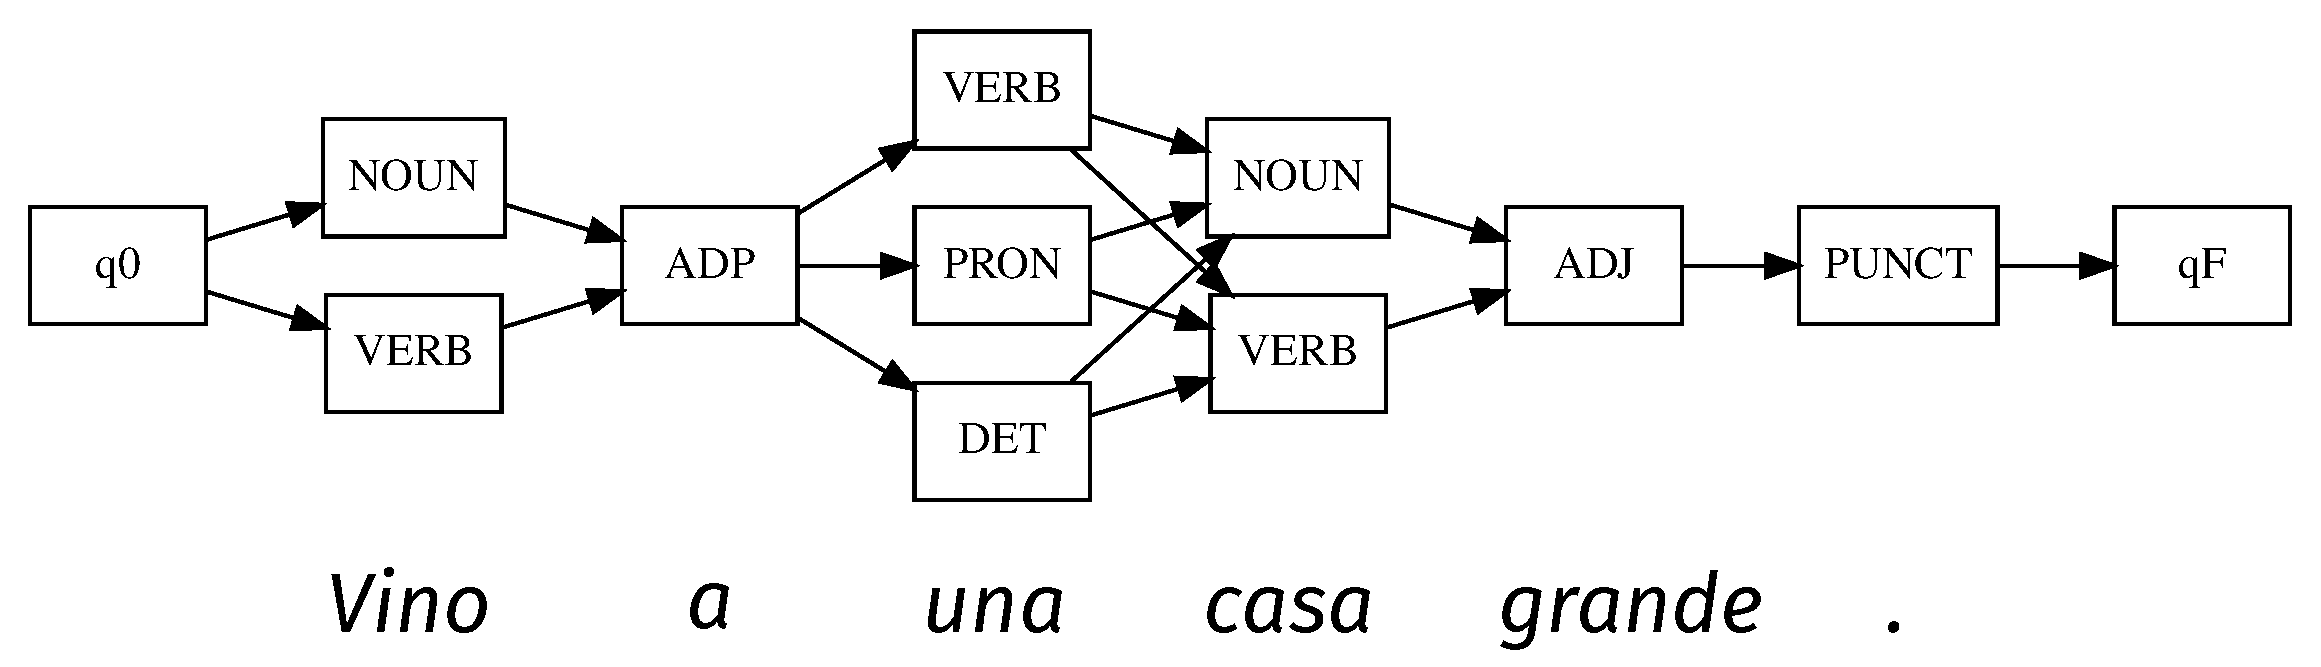
\includegraphics[width=\textwidth]{images/viterbi-1.eps}
\end{onlyenv}

\begin{onlyenv}<2>
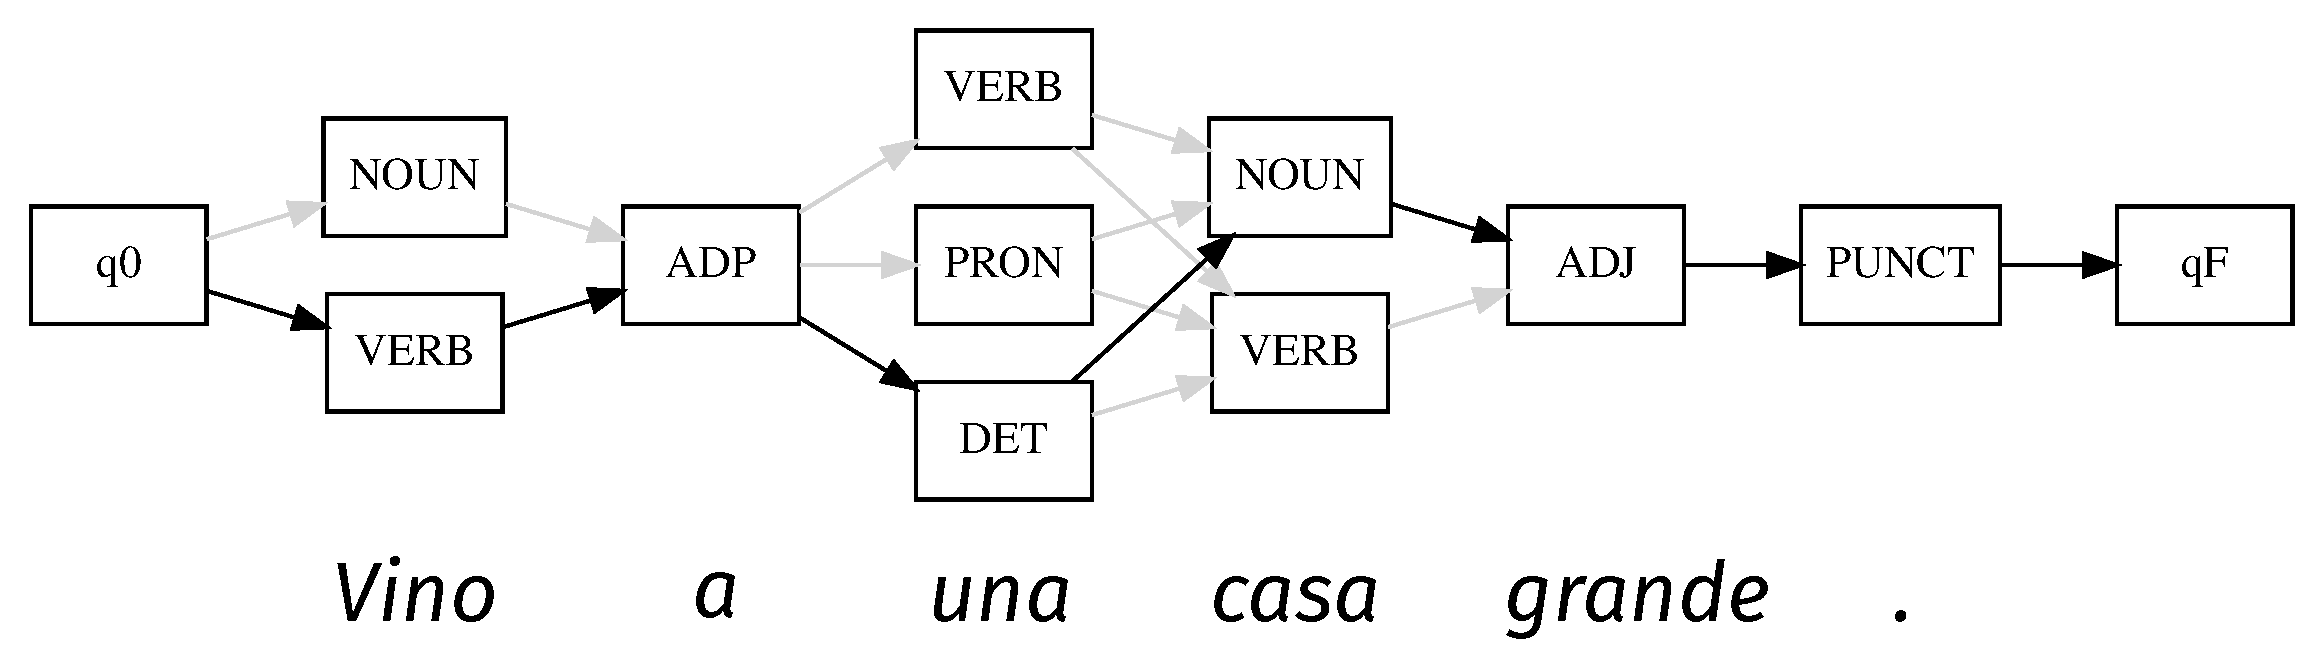
\includegraphics[width=\textwidth]{images/viterbi-2.eps}
\end{onlyenv}

\begin{itemize}
  \item Dynamic programming algorithm
  \item Find the most likely sequence of hidden states given 
    observed sequence
  \item e.g. Find POS tag sequence given words or ambiguity classes
\end{itemize}

\end{frame}


\begin{frame}{Decoding}

\begin{center}

\begin{onlyenv}<1>
  \emph{Vino a una casa grande.}
  %Vino<noun>/<verb> a<pr> una<det>/<prn>/<verb> casa<noun>/<verb> grande<adj> .<sent> 
  ~\\
  ~\\
  
  \scalebox{0.7}{
    \begin{tabular}{|l|r|r|r|r|r|r|r|}
           \multicolumn{8}{c}{{\large $\rightarrow$}}  \\
    \hline
    $q_F$ &   &   &   &   &   &   &    \\
    \hline
    VERB &  &   &   &   &   &   &    \\
    \hline
    NOUN  &   &   &   &   &   &   &    \\
    \hline
    DET &   &   &   &   &   &   &    \\
    \hline
    PRON  &   &   &   &   &   &   &    \\
    \hline
    ADP &   &   &   &   &   &   &    \\
    \hline
    ADJ  &   &   &   &   &   &   &    \\
    \hline
    PUNCT  &   &   &   &   &   &   &   \\
    \hline
          & VERB/NOUN & ADP & DET/PRON/VERB & NOUN/VERB & ADJ & PUNCT & \\
    \hline
          & \emph{Vino} & \emph{a} & \emph{una} & \emph{casa} & \emph{grande} & . & \\
    \hline
    \end{tabular}
  }
\end{onlyenv}
 
%%%%%%%%%%%%%%%%%%%%%%%%%%%%%%%%%%%%%%%%%%%%%%%%%%%%%%%%%%%%%%%%%%%%%

\begin{onlyenv}<2>

  \scalebox{0.7}{
    \begin{tabular}{|l|r|r|r|r|r|r|r|}
           \multicolumn{8}{c}{{\large $\rightarrow$}}  \\
    \hline
    $q_F$ &   &   &   &   &   &   &    \\
    \hline
    VERB & 0.15, $q_0$ &   &   &   &   &   &    \\
    \hline
    NOUN  & 0.0, $q_0$ &   &   &   &   &   &    \\
    \hline
    DET &   &   &   &   &   &   &    \\
    \hline
    PRON  &   &   &   &   &   &   &    \\
    \hline
    ADP &   &   &   &   &   &   &    \\
    \hline
    ADJ  &   &   &   &   &   &   &    \\
    \hline
    PUNCT  &   &   &   &   &   &   &   \\
    \hline
          & VERB/NOUN & ADP & DET/PRON/VERB & NOUN/VERB & ADJ & PUNCT & \\
    \hline
          & \emph{Vino} & \emph{a} & \emph{una} & \emph{casa} & \emph{grande} & . & \\
    \hline
    \end{tabular}
  }

{\small
\begin{itemize}
  \item = P(VERB,PUNCT) * P(VERB, VERB/NOUN) = 0.75 * 0.2 = 0.15
  \item = P(NOUN,PUNCT) * P(NOUN, VERB/NOUN) = 0.0 * 0.67 = 0.0
\end{itemize}
}

\end{onlyenv}


%%%%%%%%%%%%%%%%%%%%%%%%%%%%%%%%%%%%%%%%%%%%%%%%%%%%%%%%%%%%%%%%

\begin{onlyenv}<3>

  \scalebox{0.7}{
    \begin{tabular}{|l|r|r|r|r|r|r|r|}
           \multicolumn{8}{c}{{\large $\rightarrow$}}  \\
    \hline
    $q_F$ &   &   &   &   &   &   &    \\
    \hline
    VERB & 0.15, $q_0$ &   &   &   &   &   &    \\
    \hline
    NOUN  & 0.0, $q_0$ &   &   &   &   &   &    \\
    \hline
    DET &   &   &   &   &   &   &    \\
    \hline
    PRON  &   &   &   &   &   &   &    \\
    \hline
    ADP &   & 0.06, VERB  &   &   &   &   &    \\
    \hline
    ADJ  &   &   &   &   &   &   &    \\
    \hline
    PUNCT  &   &   &   &   &   &   &   \\
    \hline
          & VERB/NOUN & ADP & DET/PRON/VERB & NOUN/VERB & ADJ & PUNCT & \\
    \hline
          & \emph{Vino} & \emph{a} & \emph{una} & \emph{casa} & \emph{grande} & . & \\
    \hline
    \end{tabular}
  }

{\small
\begin{itemize}
  \item = P(ADP,VERB) * P(ADP, ADP) * P(PATH) = 0.4 * 1.0 * 0.15 = 0.06
  \item = P(ADP,NOUN) * P(ADP, ADP) * P(PATH) = 0.16 * 1.0 * 0.0 = 0
\end{itemize}
}

\end{onlyenv}

%%%%%%%%%%%%%%%%%%%%%%%%%%%%%%%%%%%%%%%%%%%%%%%%%%%%%%%%%%%%%%%%

\begin{onlyenv}<4>

  \scalebox{0.7}{
    \begin{tabular}{|l|r|r|r|r|r|r|r|}
           \multicolumn{8}{c}{{\large $\rightarrow$}}  \\
    \hline
    $q_F$   &             &             &   &   &   &   &    \\
    \hline
    VERB    & 0.15, $q_0$ &             & 0.0, ADP  &   &   &   &    \\
    \hline
    NOUN    & 0.0, $q_0$  &             &   &   &   &   &    \\
    \hline
    DET     &             &             & 0.009, ADP   &   &   &   &    \\
    \hline
    PRON    &             &             & 0.0, ADP  &   &   &   &    \\
    \hline
    ADP     &             & 0.06, VERB  &   &   &   &   &    \\
    \hline
    ADJ     &             &             &   &   &   &   &    \\
    \hline
    PUNCT   &             &             &   &   &   &   &   \\
    \hline
          & VERB/NOUN & ADP & DET/PRON/VERB & NOUN/VERB & ADJ & PUNCT & \\
    \hline
          & \emph{Vino} & \emph{a} & \emph{una} & \emph{casa} & \emph{grande} & . & \\
    \hline
    \end{tabular}
  }

{\tiny
\begin{itemize}
  \item = P(DET,ADP) * P(DET, DET/PRON/VERB) * P(PATH) = 0.6 * 0.25 * 0.06 = 0.009
  \item = P(PRON,ADP) * P(PRON, DET/PRON/VERB) * P(PATH) = 0.0 * 0.0 * 0.06 = 0.0
  \item = P(VERB,ADP) * P(VERB, DET/PRON/VERB) * P(PATH) = 0.0 * 0.0 * 0.06 = 0.0
\end{itemize}
}

\end{onlyenv}

%%%%%%%%%%%%%%%%%%%%%%%%%%%%%%%%%%%%%%%%%%%%%%%%%%%%%%%%%%%%%%%%

\begin{onlyenv}<5>

  \scalebox{0.7}{
    \begin{tabular}{|l|r|r|r|r|r|r|r|}
           \multicolumn{8}{c}{{\large $\rightarrow$}}  \\
    \hline
    $q_F$   &             &             &   &   &   &   &    \\
    \hline
    VERB    & 0.15, $q_0$ &             & 0.0, ADP  & 0.0, DET*  &   &   &    \\
    \hline
    NOUN    & 0.0, $q_0$  &             &           & 0.006, DET   &   &  &    \\
    \hline
    DET     &             &             & 0.009, ADP   &   &   &   &    \\
    \hline
    PRON    &             &             & 0.0, ADP  &   &   &   &    \\
    \hline
    ADP     &             & 0.06, VERB  &   &   &   &   &    \\
    \hline
    ADJ     &             &             &   &   &   &   &    \\
    \hline
    PUNCT   &             &             &   &   &   &   &   \\
    \hline
          & VERB/NOUN & ADP & DET/PRON/VERB & NOUN/VERB & ADJ & PUNCT & \\
    \hline
          & \emph{Vino} & \emph{a} & \emph{una} & \emph{casa} & \emph{grande} & . & \\
    \hline
    \end{tabular}
  }

{\tiny
\begin{itemize}
  \item = P(NOUN,VERB) * P(NOUN, NOUN/VERB) * P(PATH) = 0.2 * 0.67 * 0.009 = 0.001
  \item = P(VERB,VERB) * P(VERB, NOUN/VERB) * P(PATH) = 0.0 * 0.2  * 0.009 = 0.0
  \item = P(NOUN,DET) * P(NOUN, NOUN/VERB) * P(PATH) =  1.0 * 0.67 * 0.009 = 0.006
  \item = P(VERB,DET) * P(VERB, NOUN/VERB) * P(PATH) =  0.0 * 0.2  * 0.009 = 0.0
  \item = P(NOUN,PRON) * P(NOUN, NOUN/VERB) * P(PATH) = 0.0 * 0.67 * 0.009 = 0.0 
  \item = P(VERB,PRON) * P(VERB, NOUN/VERB) * P(PATH) = 0.0 * 0.67 * 0.009 = 0.0
\end{itemize}
}

\end{onlyenv}

%%%%%%%%%%%%%%%%%%%%%%%%%%%%%%%%%%%%%%%%%%%%%%%%%%%%%%%%%%%%%%%%

\begin{onlyenv}<6>

  \scalebox{0.7}{
    \begin{tabular}{|l|r|r|r|r|r|r|r|}
           \multicolumn{8}{c}{{\large $\rightarrow$}}  \\
    \hline
    $q_F$   &             &             &   &   &   &   &    \\
    \hline
    VERB    & 0.15, $q_0$ &             & 0.0, ADP  & 0.0, DET*  &   &   &    \\
    \hline
    NOUN    & 0.0, $q_0$  &             &           & 0.006, DET   &   &  &    \\
    \hline
    DET     &             &             & 0.009, ADP   &   &   &   &    \\
    \hline
    PRON    &             &             & 0.0, ADP  &   &   &   &    \\
    \hline
    ADP     &             & 0.06, VERB  &   &   &   &   &    \\
    \hline
    ADJ     &             &             &   &   &    0.001, NOUN &  &    \\
    \hline
    PUNCT   &             &             &   &   &   &   &   \\
    \hline
          & VERB/NOUN & ADP & DET/PRON/VERB & NOUN/VERB & ADJ & PUNCT & \\
    \hline
          & \emph{Vino} & \emph{a} & \emph{una} & \emph{casa} & \emph{grande} & . & \\
    \hline
    \end{tabular}
  }

{\tiny
\begin{itemize}
  \item = P(ADJ,NOUN) * P(ADJ, ADJ) * P(PATH) = 0.16 * 1.0 * 0.006 = 0.00096
  \item = P(ADJ,VERB) * P(ADJ, ADJ) * P(PATH) = 0.2 * 1.0 * 0.0 = 0.0
\end{itemize}
}

\end{onlyenv}

%%%%%%%%%%%%%%%%%%%%%%%%%%%%%%%%%%%%%%%%%%%%%%%%%%%%%%%%%%%%%%%%

\begin{onlyenv}<7>

  \scalebox{0.7}{
    \begin{tabular}{|l|r|r|r|r|r|r|r|}
           \multicolumn{8}{c}{{\large $\rightarrow$}}  \\
    \hline
    $q_F$   &             &             &   &   &   &   &    \\
    \hline
    VERB    & 0.15, $q_0$ &             & 0.0, ADP  & 0.0, DET*  &   &   &    \\
    \hline
    NOUN    & 0.0, $q_0$  &             &           & 0.006, DET   &   &  &    \\
    \hline
    DET     &             &             & 0.009, ADP   &   &   &   &    \\
    \hline
    PRON    &             &             & 0.0, ADP  &   &   &   &    \\
    \hline
    ADP     &             & 0.06, VERB  &   &   &   &   &    \\
    \hline
    ADJ     &             &             &   &   &    0.001, NOUN &  &    \\
    \hline
    PUNCT   &             &             &   &   &   & 0.001, ADJ  &   \\
    \hline
          & VERB/NOUN & ADP & DET/PRON/VERB & NOUN/VERB & ADJ & PUNCT & \\
    \hline
          & \emph{Vino} & \emph{a} & \emph{una} & \emph{casa} & \emph{grande} & . & \\
    \hline
    \end{tabular}
  }

{\tiny
\begin{itemize}
  \item = P(PUNCT,ADJ) * P(PUNCT, PUNCT) * P(PATH) = 1.0 * 1.0 * 0.001 = 0.001
\end{itemize}
}

\end{onlyenv}

%%%%%%%%%%%%%%%%%%%%%%%%%%%%%%%%%%%%%%%%%%%%%%%%%%%%%%%%%%%%%%%%%%%%%%%%%%%%%%%%%%%%%%

\begin{onlyenv}<8->

  \scalebox{0.7}{
    \begin{tabular}{|l|r|r|r|r|r|r|r|}
           \multicolumn{8}{c}{{\large $\rightarrow$}}  \\
    \hline
    $q_F$   &             &             &   &   &   &   &    \\
    \hline
    VERB    & 0.15, \alert<14>{$q_0$} &             & 0.0, ADP  & 0.0, DET*  &   &   &    \\
    \hline
    NOUN    & 0.0, $q_0$  &             &           & 0.006, \alert<11>{DET}   &   &  &    \\
    \hline
    DET     &             &             & 0.009, \alert<12>{ADP}   &   &   &   &    \\
    \hline
    PRON    &             &             & 0.0, ADP  &   &   &   &    \\
    \hline
    ADP     &             & 0.06, \alert<13>{VERB}  &   &   &   &   &    \\
    \hline
    ADJ     &             &             &   &   &    0.001, \alert<10>{NOUN} &  &    \\
    \hline
    PUNCT   &             &             &   &   &   & 0.001, \alert<9>{ADJ}  &   \\
    \hline
          & VERB/NOUN & ADP & DET/PRON/VERB & NOUN/VERB & ADJ & PUNCT & \\
    \hline
          & \emph{Vino} & \emph{a} & \emph{una} & \emph{casa} & \emph{grande} & . & \\
    \hline
    \end{tabular}
  }
\end{onlyenv}

\begin{onlyenv}<8>
PUNCT
\end{onlyenv}
\begin{onlyenv}<9>
ADJ PUNCT
\end{onlyenv}
\begin{onlyenv}<10>
NOUN ADJ PUNCT
\end{onlyenv}
\begin{onlyenv}<11>
DET NOUN ADJ PUNCT
\end{onlyenv}
\begin{onlyenv}<12>
ADP DET NOUN ADJ PUNCT
\end{onlyenv}
\begin{onlyenv}<13->
VERB ADP DET NOUN ADJ PUNCT
\end{onlyenv}

\end{center}


% step 1: PUNCT VERB = p(verb,punct) = 0.75 * 0.2 || PUNCT NOUN = p(noun,punct) = 0 * 0.67 = 0

\end{frame}

\begin{frame}{Implementation}
\begin{center}
\url{https://paste2.org/HMgn7amd}
~\\
~\\
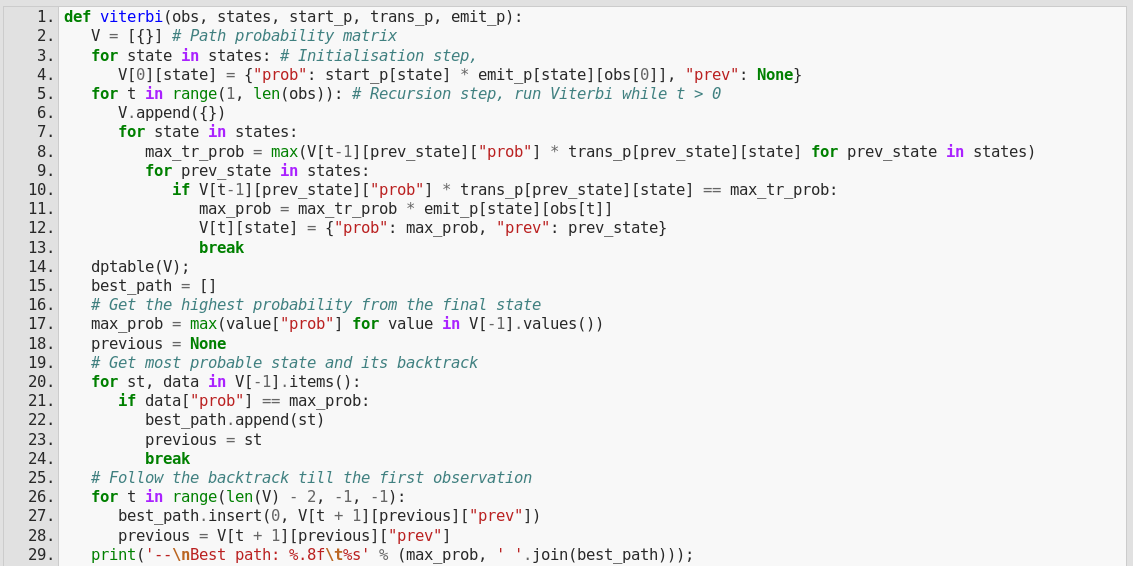
\includegraphics[width=\textwidth]{images/viterbi-wp.png}
\end{center}

\end{frame}

\begin{frame}{Extensions}

\begin{itemize}
  \item Trigrams
  \begin{itemize}
     \item Instead of conditioning on previous tag, condition on previous two
  \end{itemize}
  \item Unknown words
  \begin{itemize}
     \item Incorporate suffixes into the tags
  \end{itemize} 
  \item Backoff 
  \begin{itemize}
    \item If the bi-/tri-gram hasn't been seen, backoff to lower order model
  \end{itemize}
  \item Capitalisation
  \begin{itemize}
    \item Use capitalisation features 
  \end{itemize}
\end{itemize}

% downsides
% Hard to add new features

\end{frame}


%%%%%%%%%%%%%%%%%%%%%%%%%%%%%%%%%%%%%%%%%%%%%%%%%%%%%%%%%%%%%%%%%%%%%%%%%%%%%%%
% Averaged Perceptron
\begin{frame}
\centering
{\LARGE {\bf Averaged perceptron} }
\end{frame}

\begin{frame}
% discriminative model
% beautifully simple

\textbf{A binary perceptron:}
\begin{center}
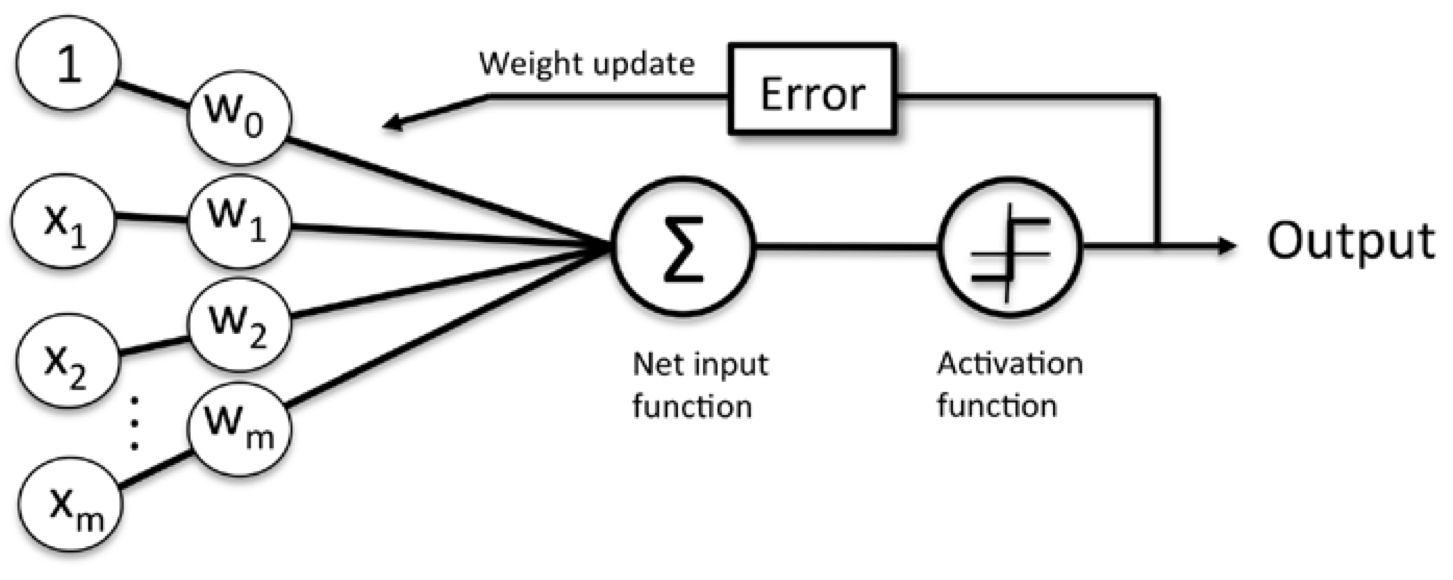
\includegraphics[width=0.8\textwidth]{images/perceptron.png}
\end{center}

\begin{itemize}
  \item Discriminative model ... find the category, not the distribution
  \item Beautifully simple
\end{itemize}

\begin{center}
 \url{github.com/ftyers/conllu-perceptron-tagger}
\end{center}

\end{frame}

\begin{frame}{Training}

\begin{center}
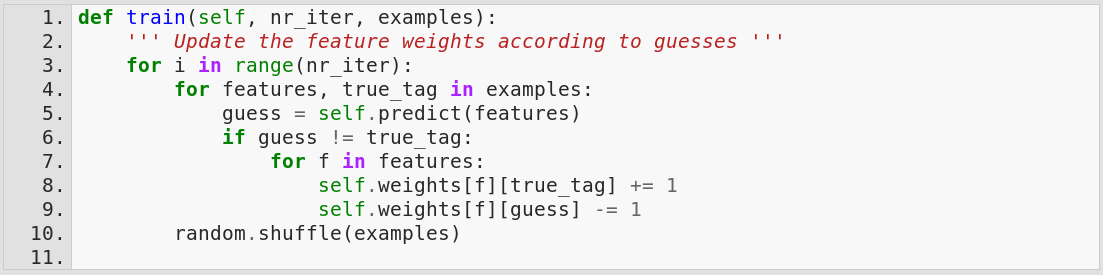
\includegraphics[width=\textwidth]{images/perceptron-train.png}
\end{center}

\begin{itemize}
  \item We iterate through the whole training data $n$ times
  \item For each tag we try and predict the value
  \begin{itemize}
    \item If we get it wrong, we increase the weight of the features for the correct class
  \end{itemize}
\end{itemize}

% loop
% averaging
% training from predictions

\end{frame}

\begin{frame}{Features}

%    add('i suffix', word[-3:])
%    add('i pref1', word[0])
%    add('i-1 tag', prev)
%    add('i-2 tag', prev2)
%    add('i tag+i-2 tag', prev, prev2)
%    add('i word', context[i])
%    add('i-1 tag+i word', prev, context[i])
%    add('i-1 word', context[i-1])
%    add('i-1 suffix', context[i-1][-3:])
%    add('i-2 word', context[i-2])
%    add('i+1 word', context[i+1])
%    add('i+1 suffix', context[i+1][-3:])
%    add('i+2 word', context[i+2])

\begin{center}
\begin{tabular}{llllll}
Vino & a & una & casa & grande & . \\
$i-2$ & $i-1$ & $i$ & $i+1$ & $i+2$ & $i+3$ \\
\end{tabular}
\end{center} 
~\\

\begin{columns}
\begin{column}{0.5\textwidth}

\begin{itemize}
  \item Specify whatever features you want,
  \item Easy to add new ones!
\end{itemize}

\end{column}
\begin{column}{0.5\textwidth}

\scalebox{0.9}{
  \centering
  \begin{tabular}{|lll|}
  \hline
  $i$  & Trigram suffix  & una \\
  $i$  & Unigram prefix  & u \\
  $i-1$ & Tag & ADP \\
  $i-2$ & Tag & VERB \\
  %  Tag $i$ + tag $i-2$ & &  \\
  $i$ &  Word  & una \\
  $i-1$, $i$ &  Tag, Word  & ADP + una \\
  $i-1$ & Word & a \\
  $i-1$ & Trigram suffix & a \\
  $i-2$ & Word & Vino \\
  $i+1$ & Word  & casa \\
  $i+1$ & Trigram suffix  & asa \\
  $i+2$ &  Word  & grande \\
  \hline
  \end{tabular}
}
\end{column}
\end{columns}


\end{frame}

\begin{frame}{Averaging}

\textbf{Problem:}
\begin{itemize}
  \item In later iterations it changes the weights a lot for the last few
    samples it is getting wrong
  \item \ldots overfitting
\end{itemize}

\textbf{Solution:}
\begin{itemize}
  \item Average the weights over the iterations
\end{itemize}

\end{frame}

\begin{frame}{Dictionary}

Given the amount of unambiguous words:
\begin{itemize}
  \item Make a dictionary
  \item When you see the word, output it
  \item But have a frequency threshold, e.g. 20
\end{itemize}
%, it also makes sense to make a dictionary
%of those and when we see them just output that tag.

\end{frame}

\begin{frame}{Prediction}

\begin{center}
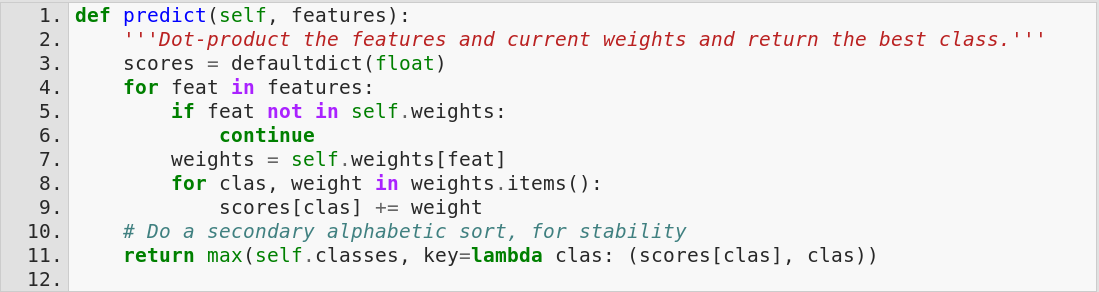
\includegraphics[width=\textwidth]{images/perceptron-predict.png}
\end{center}

\begin{itemize}
  \item For each class (POS), add the weights of the features we've seen
  \item Take the class with the maximum weight
\end{itemize}

\end{frame}

%%%%%%%%%%%%%%%%%%%%%%%%%%%%%%%%%%%%%%%%%%%%%%%%%%%%%%%%%%%%%%%%%%%%%%%%%%%%%%%

\begin{frame}

\centering
{\LARGE {\bf Discussion} }

\end{frame}

\begin{frame}{Comparison of approaches}


\begin{onlyenv}<1>
\begin{center}
\begin{tabular}{|l|c|c|}
 \hline
   & {\Large \textbf{+}} & {\Large \textbf{-}}  \\
 \hline
\textbf{CG} & Start from scratch & Tagset not learnt \\
\textbf{HMM} & Model distribution & Hard to incorporate feats \\
\textbf{Perceptron} & Easy to incorporate feats & No $n$-best  \\
 \hline
\end{tabular}
\end{center}
% CG -- can start from scratch, but tagsets can be a problem, no explicit lexical info
% HMM -- can make n-best list
% perceptron -- more robust, easier to add features to

All techniques can reach 97\% token accuracy.
\begin{itemize}
  \item Great ... but 57\% full-sentence accuracy.
\end{itemize}
\end{onlyenv}
\begin{onlyenv}<2>
% all taggers report around 97% accuracy [refs]
% getting beyond 97% ?
%% Chris Manning (2011) "Part-of-Speech Tagging from 97% to 100%: Is It Time for Some Linguistics?"

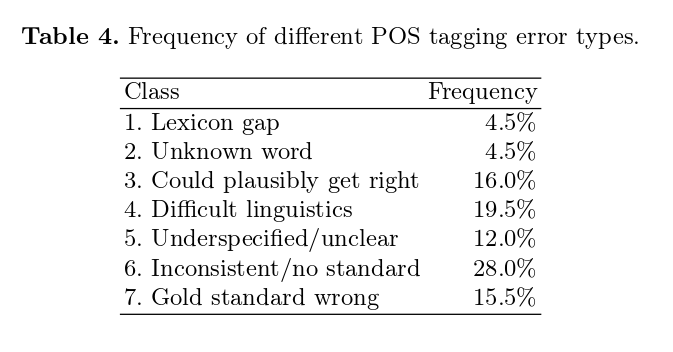
\includegraphics[width=\textwidth]{images/manning-errors.png}
~\\
Chris Manning (2011) ``Part-of-Speech Tagging from 97\% to 100\%: Is It Time for Some Linguistics?"
\end{onlyenv}

%% At first glance, current part-of-speech taggers work rapidly and reliably, with
%per-token accuracies of slightly over 97% [1–4]. Looked at more carefully, the
%story is not quite so rosy. This evaluation measure is easy both beca
%use it is measured per-token and because you get points for every punctuation mark and
%other tokens that are not ambiguous. It is perhaps more realistic to look at the
%rate of getting whole sentences right, since a single bad mistake in a sentence
%can greatly throw off the usefulness of a tagger to downstream tasks such as
%dependency parsing. Current good taggers have sentence accuracies around 55–
%57%, which is a much more modest score.

\end{frame}


%%%%%%%%%%%%%%%%%%%%%%%%%%%%%%%%%%%%%%%%%%%%%%%%%%%%%%%%%%%%%%%%%%%%%%%%%%%%%%%

% How much data ?

\begin{frame}{How much time and effort ?}

\begin{center}
 Annotation time vs. rule-writing time
\end{center}

\begin{itemize}
   \item Hand annotation: 8000--10000 tokens/month 
   \begin{itemize}
     \item 50--100k tokens = 6--12 months
   \end{itemize}
   \item Rule-based:
   \begin{itemize}
    \item  Morphological analyser: 3--6 months
    \item  Constraint grammar: 3--6 months
   \end{itemize}
\end{itemize}

Approaching a new language, depends on what you like doing more.
% annotation time vs. rule-writing time

% Huldén 20 hours / 148 rules / 113 generic, 35 for wordforms [working from a devel. corpus]
% Tyers 1 month / 299 rules [working from nothing]

% 8000--10000 tokens/month = ~50-60 tokens/hour

\end{frame}

% Combination/voting

\begin{frame}{Tagger combination}


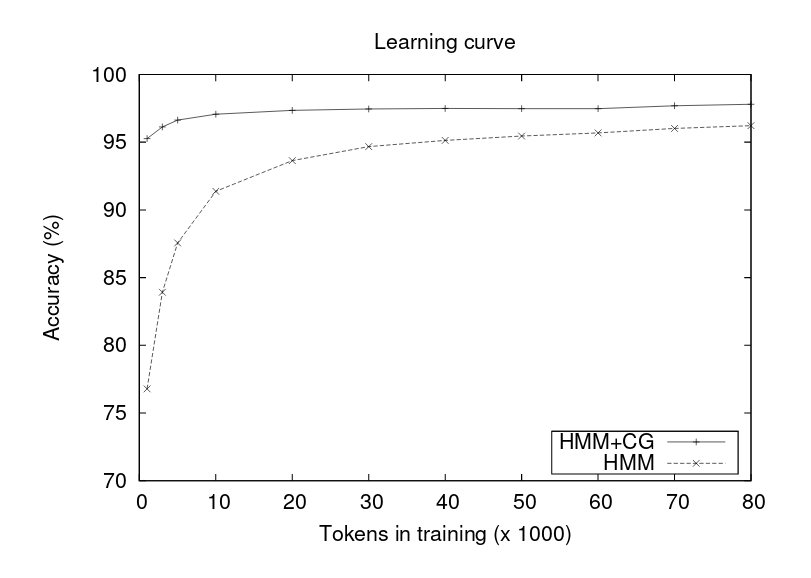
\includegraphics[width=0.49\textwidth]{images/mans-huldren-tagger-chart.png}
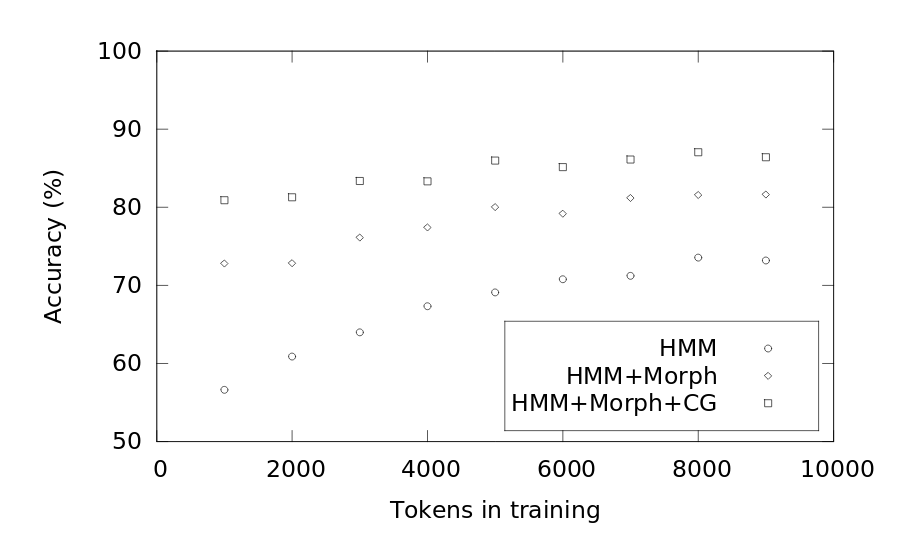
\includegraphics[width=0.49\textwidth]{images/fran-rob-tagger-graph.png}

\begin{itemize}
  \item Voting systems 
  \item Combine systems that make complementary errors
\end{itemize}

\end{frame}


\begin{frame}{Some taggers}
% some state of the art systems

% specifically for russian:
%pymorphy2, pymystem3?

\textbf{Russian:}
\begin{itemize}
  \item {\tt pymorphy2}
  \item {\tt mystem3}
\end{itemize}

\textbf{Trainable:}
\begin{itemize}
  \item HunPos (HMM, OCaml)
  \item UDPipe/MorphoDiTa (Av. Perceptron, C++)
  \item MarMot (CRF, Java)
  \item NLTK (various, Python)
\end{itemize}


\end{frame}

% error analysis: http://machinelearningtext.pbworks.com/w/file/fetch/48157747/CICLing2011-manning-tagging.pdf

%\begin{frame}
 
%\end{frame}

\begin{frame}{Practicals}
\url{https://ftyers.github.io/2017-КЛ\_МКЛ/practicals/disambiguation.html}

\begin{itemize}
  \item \textbf{Tagger comparison}:
  \begin{itemize}
     \item Compare three taggers on a language/domain of your choice
  \end{itemize}
  \item \textbf{Constraint grammar}: 
  \begin{itemize}
     \item Select a small text (one paragraph) in a language of your choice
     \item Analyse it with a morphological analyser
     \item Resolve as much of the ambiguity as you can
  \end{itemize}
  \item \textbf{Perceptron tagger}:
  \begin{itemize}
     \item Download \url{https://github.com/ftyers/conllu-perceptron-tagger}
     \item Run it on a language from Universal Dependencies
     \item Improve it so that you get better performance
     \begin{itemize}
       \item Add support for morphological features
       \item Try tweaking other features
     \end{itemize}
  \end{itemize}
\end{itemize}

\end{frame}

\end{document}
